\subsection{Organisation d'une application basée sur une telle architecture}
\paragraph{}
Dans une application, les besoins fonctionnels et non fonctionnels peuvent être différents selon que l'on s'intéresse à ses composantes de lecture ou d'écriture.
Dans le cas d'une IHM, il est important que l'information que l'on souhaite afficher soit disponible à l'utilisateur sans qu'il n'ait à croiser lui-même différentes informations présentes sur différents écrans.
Il est alors nécessaire d'aggréger et de filtrer les données et donc de les dénormaliser lorsqu'elles sont destinées à la consultation.
D'autre part, lorsqu'un utilisateur souhaitera exécuter une action d'écriture, l'ensemble des données manipulées sera plus réduit et la problématique ne sera plus la même.
La complexité se trouvera plutôt dans la vérification du respect de règles et il sera nécessaire d'utiliser des entités d'association pour ce faire.
Ainsi, on privilégie dans ce cas une normalisation des données ainsi que leur intégrité.
On voit alors que les besoins en écriture sont globalement transactionnels et une garantie de cohérence des données ainsi que leur normalisation est nécessaire, tandis qu'en lecture, les besoins sont davantage en dénormalisation des données ainsi qu'en scalabilité.
\paragraph{}
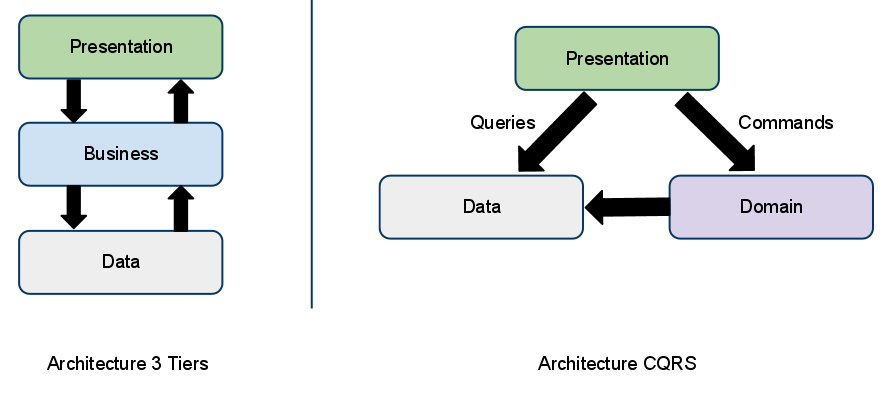
\includegraphics[scale=0.4]{Figures/Chapter3/architecture/tiersvscqrs.png}
Par opposition à une architecture du type 3 tiers, dont les services permettant d'accéder aux données se confondent avec ceux qui vont agir sur ces même données, l'architecture CQRS sépare volontairement les composants requêtant les données de ceux qui les modifient.
Une telle séparation facilite l'organisation de l'application puisque des composants différents sont utilisés pour des problématiques différentes, mais permet aussi de profiter des avantages de différentes technologies sur ces composants et ainsi d'optimiser les performances de l'application.
\paragraph{}
L'architecture CQRS se base sur plusieurs concepts tirés du Domain Driven Design (DDD).
Il me semble important, avant de détailler le contenu des différentes couches formant cette architecture, de clarifier quelques termes, que j'ai appris à connaître au cours de mon stage.

\subsubsection{Les concepts tirés du Domain Driven Design}
\label{subs:Les concepts tirés du Domain Driven Design}
\paragraph{Le domaine}
\label{par:Le domaine}
Le domaine est la zone où est concentré toute la connaissance métier de l'application.
On y trouve ainsi les objets nécessaires pour appliquer les règles métiers et pour appliquer les contrôles nécessaires à chaque actions, des agrégats et des services notamment.
\paragraph{Les aggrégats}
\label{par:Les aggrégats}
Un aggrégat est un objet modifiable lors d'une transaction.
Il est généralement repésenté par une classe possédant un identifiant unique dans toute l'application mais on peut aussi trouver des représentations d'aggrégats via plusieurs classes.
Dans ce second cas, une d'entre elle est dite classe racine ("root class") et tout accès à l'aggrégat par l'extérieur se fait via cette classe et toutes les autres restent interne à l'agrégat.
Ces classes contiennent la logique du domaine (\ref{par:Le domaine}) et permettent d'effectuer des contrôles.
\paragraph{Les repositories (ou dépôts)}
\label{par:Les repositories (ou dépôts)}
Les différentes instances des aggrégats sont stockées dans un objet appelé repository (dépôt en français).
Ces objets servent d'intermédiaires entre le domaine (\ref{par:Le domaine}) et la base de donnée.
On retrouve dans ces objets des méthodes du type 'save' qui permet de sauvegarder les changements relatifs à un aggrégat ou 'getById' qui permet de récupérer un aggrégat particulier.


%-------------------------------------------------------------------------
\subsubsection{La couche de modification des données: Command}
\label{subs:La couche de modification des données: Command}
\paragraph{}
Cette couche concentre toutes les modifications des données, qu'il s'agisse de création, de suppression ou de mise à jour.
Une commande représente une action destinée à être exécutée, une intention, et n'est pas une simple demande d'altération de donnée.
Généralement, une commande est représentée comme un appel de méthode encapsulée dans un objet; elle porte un nom explicite et ses champs contiennent les différents paramètres de l'action.
Dans le cas de l'espace recruteur du site Cadremploi.fr, les commandes ont pour but d'enregistrer les altérations effectuées par les événements côté client, et on retrouve des commandes nommées 'ModifierTitrePosteCommand' ou 'PayerOffreCommand' par exemple, permettant de modifier le titre du poste dans l'annonce ou de payer l'offre saisie respectivement.
De tels noms sont ainsi très expressifs et permettent de clarifier la cause de la modification des données.
\paragraph{}
Une commande récupère via des repositories les agrégats qu'elle vise.
Via les informations contenues dans ces agrégats et potentiellement avec différents services, les contrôles nécessaires à la validation de la commande peuvent être appliqués.
Une fois que les différents contrôles sur la commande faits, on applique son effet sur l'aggrégat, ce qui génère des événements de modification.
Les découpages et cette logique permettent de maîtriser l'impact de chaque action sur le système.
\paragraph{}
Les méthodes de commandes prennent ainsi en paramètre des identifiants d'entités ainsi que des valeurs simples.
Elles ne doivent rien renvoyer mais peuvent générer des exceptions.
La mise en commun des patterns CQRS et Event Sourcing demande l'envoi des événements générés dans un bus en même temps que l'enregistrement des modifications sur l'aggrégat.
Ces événements seront écoutés et utilisés pour la construction de la seconde couche de ce pattern, la couche de lecture des données.

%-------------------------------------------------------------------------
\subsubsection{La couche de lecture des données: Query}
\label{subs:La couche de lecture des données: Query}
\paragraph{}
La partie Query de ce modèle se base sur le fait que les objets du \ref(subs:Le domaine){domaine} sont volumineux et qu'il est possible de s'en passer.
Cette couche fonctionne ainsi uniquement en lecture seule et aucune modification n'est apportée aux données.
En effet le besoin représenté ici est celui d'une lecture dans un cas d'utilisation bien précis, l'objectif est d'aller extrêmement vite.
Le pattern Query consiste alors à exécuter une requête précise en base et de restituer un objet de type Data Transfer Object (DTO) concis qui pourra être utilisé directement.
Cela signifie que les contrôles sont réduits au minimum et que les DTOs utilisés sont des objets représentant exactement et uniquement le besoin en lecture, généralement des besoins IHM.
Cette méthode permet de récupérer seulement les données dont on a besoin en une fois, en se passant ainsi de parcourir plusieurs tables à travers desquelles les données seraient éparpillées.
\paragraph{}
Les projections sont des objets écoutant des événements particuliers émanant des modifications venant de la couche de modification des données.
Leur but est de retirer certaines informations particulières de ces événements de manière à construire les DTO qui seront utilisés dans la couche lecture.
Les projections écoutent alors les événements apparaissant dans le bus de manière asynchrone et répercutent les changements qu'ils demandent, mettant ainsi à jour la couche de lecture symétriquement à la couche d'écriture.

\paragraph{}
\label{par:Organisation conclusion}
L'architecture CQRS possède plusieurs avantages blablaabl
